\documentclass[11pt]{article}

\usepackage[margin=1in]{geometry}
\usepackage{amsmath,amssymb,amsthm,mathtools}
\usepackage{graphicx}
\usepackage{microtype}
\usepackage[hidelinks]{hyperref}
\usepackage{xcolor}

\newtheorem{theorem}{Theorem}
\newtheorem{lemma}[theorem]{Lemma}
\newtheorem{corollary}[theorem]{Corollary}
\newtheorem{remark}[theorem]{Remark}
\newcommand{\C}{\mathbb C}
\newcommand{\N}{\mathbb N}
\newcommand{\dd}{\,d}
\newcommand{\Lb}{\mathbb L_b}
\newcommand{\Lmn}{\mathbb L_{m,n}}
\newcommand{\pcheck}{\check p}
\newcommand{\Rclass}{\widetilde{\mathcal R}}

\title{Leray Boundedness Without Uniform Continuity\\
\large A full candidate solution to the omitted case in arXiv:2405.12753}
\author{Automated mathematics run \texttt{fa\_banach\_001}, lane 11}
\date{23 July 2026}

\begin{document}
\maketitle

\begin{center}
\fbox{\parbox{0.92\textwidth}{\textbf{Status.}
Full solution candidate, likely valid, awaiting human review.
For the source class of convex Reinhardt domains, the proof removes the
uniform-continuity hypothesis and completes the Leray-transform dichotomy:
boundedness holds exactly when
\(\kappa_3/(\kappa_1\kappa_2)\) is bounded above and bounded away from zero.}}
\end{center}

\section{Source problem}

The source is A.~Chatterjee, \emph{The Laplace and Leray transforms on some
(weakly) convex domains in \(\C^2\)}, arXiv:2405.12753
\cite{Chatterjee}.  Its Theorem 1.4 considers the densely defined Leray
transform \(\Lb\) on a domain \(\Omega\in\Rclass\), with respect to the
canonical boundary Monge--Amp\`ere measure \(\mu_\Omega\).  It proves:
\begin{enumerate}
\item boundedness if the curvature ratio
  \[
    K_\Omega=\frac{\kappa_3}{\kappa_1\kappa_2}
  \]
  is uniformly continuous and bounded away from zero; and
\item unboundedness if \(K_\Omega\) is not bounded above or is not bounded
  away from zero.
\end{enumerate}
The sole remaining case is therefore that \(K_\Omega\) is bounded above and
away from zero but has no continuous extension to the axes.  Section 4.3 of
the current source PDF isolates this case and explains why the regular
variation argument used in the positive theorem no longer applies.

\begin{figure}[ht]
\centering

\includegraphics[width=0.98\textwidth]{figures/open_problem_crop.png}
\caption{The exact omitted case, source Section 4.3, page 20.}
\end{figure}

In the source parametrization,
\[
\begin{aligned}
r_1(s)&=b_1\exp\left(-\int_s^1\frac{\dd t}{t\pcheck(t)}\right),\\
r_2(s)&=b_2\exp\left(-\int_0^s\frac{\dd t}{(1-t)\pcheck(t)}\right),
\qquad 0<s<1,
\end{aligned}
\]
where \(\pcheck:(0,1)\to(1,\infty)\) is the exponent function.  The dual
domain has
\[
 r_1^*(s)=\frac{s}{r_1(s)},\qquad
 r_2^*(s)=\frac{1-s}{r_2(s)}.
\]
The source notes that its omitted geometric case makes \(\pcheck\) remain
bounded away from \(1\) and infinity but permits it to oscillate without an
endpoint limit.  We prove boundedness using only those two bounds.

\section{Proof intuition}

The source analyzes each monomial mode by endpoint regular variation.  That
is more asymptotic information than boundedness needs.  For mode \((m,n)\),
the primal density
\[
 F=r_1^{2m}r_2^{2n}
\]
and its dual density
\[
 F^*=(r_1^*)^{2m}(r_2^*)^{2n}
\]
have their maximum at the same point \(s_0=m/(m+n)\).  Moreover,
\(FF^*=s^{2m}(1-s)^{2n}\), the ordinary beta kernel.

The logarithmic derivative of \(F\) is \(1/\pcheck(s)\) times the
logarithmic derivative of that beta kernel; for \(F^*\), the multiplier is
\(1-1/\pcheck(s)\).  Uniform upper and lower bounds on \(\pcheck\) therefore
dominate each normalized density by a fixed positive power of the beta
kernel.  Its integral has width
\(\sqrt{(m+1)(n+1)}/(m+n+1)^{3/2}\).  The product of the primal and dual
widths cancels exactly against the factorial coefficient in the source
rank-one norm formula.  This gives a uniform mode bound without requiring
any limit of \(\pcheck\).

\section{Source rank-one criterion}

The source decomposes \(L^2(b\Omega,\mu_\Omega)\) orthogonally into monomial
subspaces.  Its Lemma 3.5 states that, for \(m,n\geq0\),
\begin{equation}\label{eq:source-norm}
 \|\Lmn\|_{\mu_\Omega}^2
 =\gamma_{m,n}^2
 \left(\int_0^1r_1(s)^{2m}r_2(s)^{2n}\dd s\right)
 \left(\int_0^1r_1^*(s)^{2m}r_2^*(s)^{2n}\dd s\right),
\end{equation}
where
\[
 \gamma_{m,n}=\frac{(m+n+1)!}{m!\,n!}.
\]
It also states that \(\Lb\) is bounded if and only if these rank-one norms
are uniformly bounded, in which case \(\Lb\) is a bounded projection onto
\(\mathcal H^2(\Omega,\mu_\Omega)\).

\begin{figure}[ht]
\centering
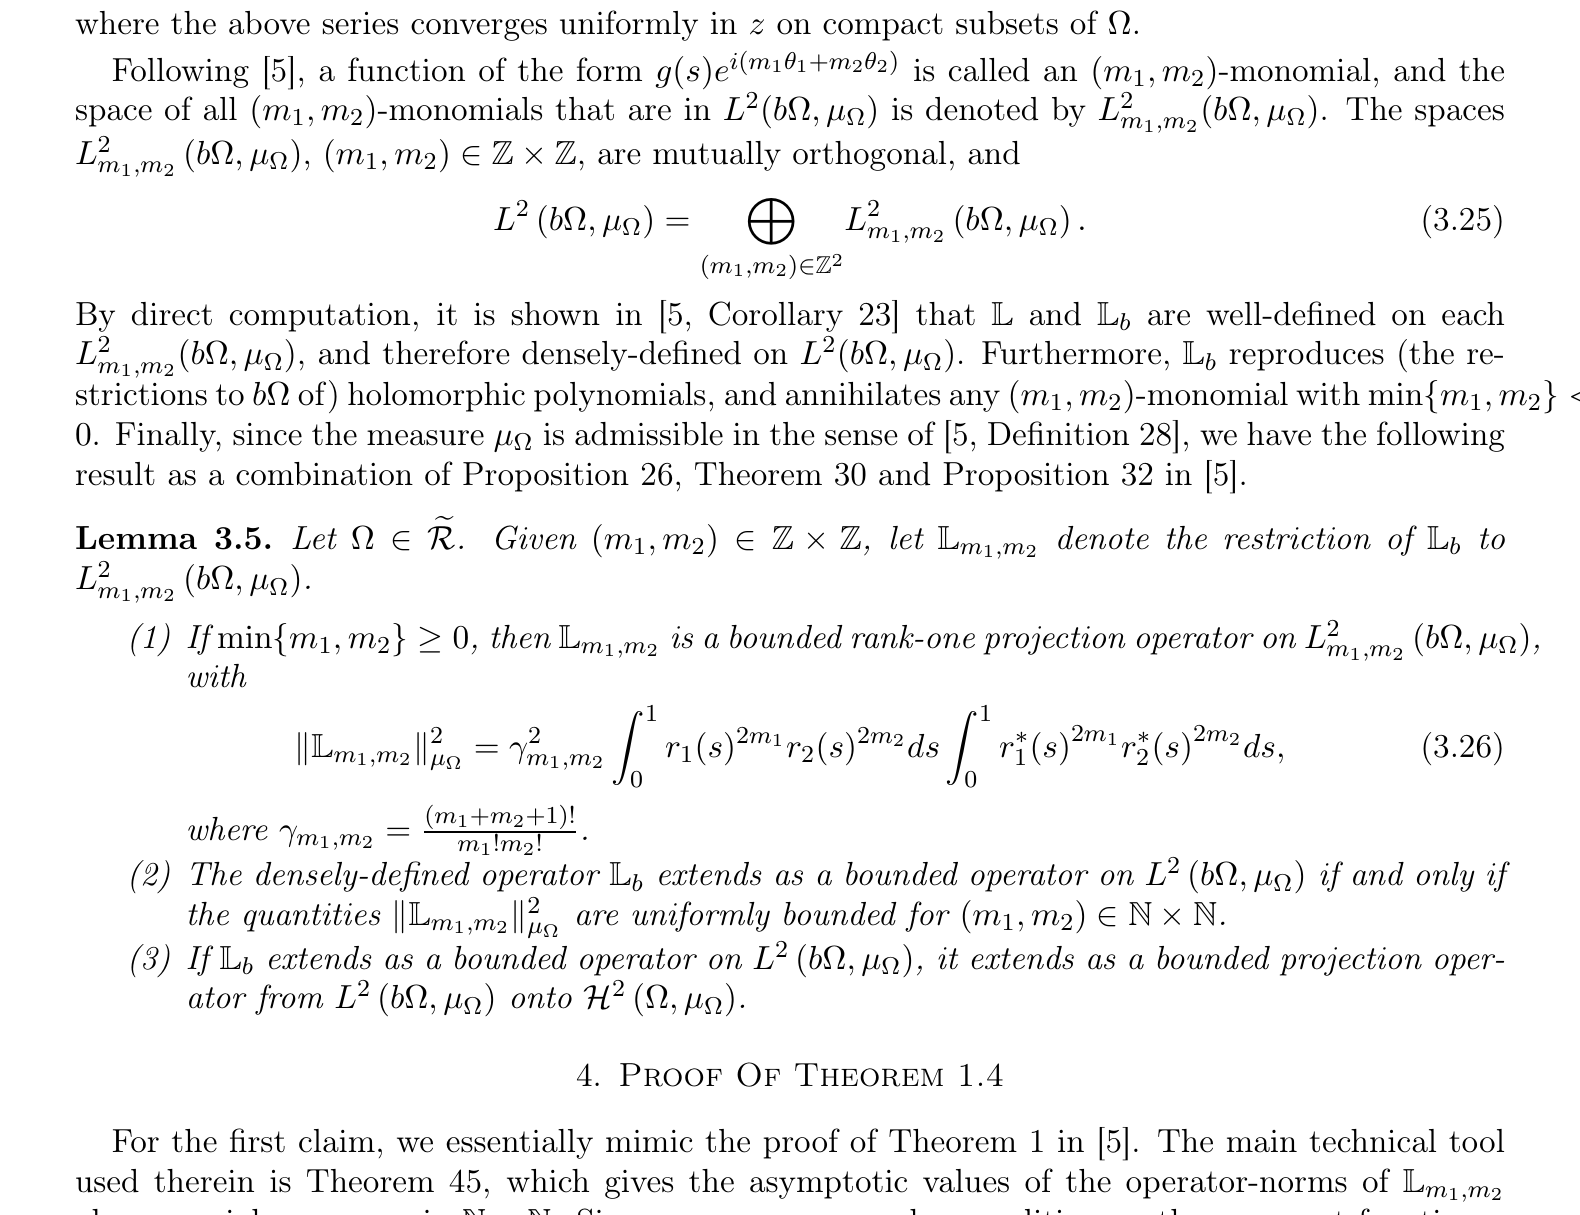
\includegraphics[width=0.98\textwidth]{figures/rank_one_criterion_crop.png}
\caption{The rank-one norm formula and boundedness criterion, source
Lemma 3.5, page 16.}
\end{figure}

\section{Two uniform estimates}

We use the conventions \(0^0=1\) and \(0\log0=0\).

\begin{lemma}[Normalized beta width]\label{lem:beta}
For each fixed \(c>0\), there is \(C_c<\infty\) such that, for all
\(m,n\geq0\), \(M=m+n>0\), and
\[
 B_{m,n}(s)=s^{2m}(1-s)^{2n},\qquad s_0=\frac mM,
\]
one has
\begin{equation}\label{eq:beta-width}
 J_c(m,n):=\int_0^1
 \left(\frac{B_{m,n}(s)}{B_{m,n}(s_0)}\right)^c\dd s
 \leq C_c\frac{\sqrt{(m+1)(n+1)}}{(M+1)^{3/2}}.
\end{equation}
\end{lemma}

\begin{proof}
The beta integral gives the exact identity
\begin{equation}\label{eq:J-exact}
 J_c(m,n)=
 \frac{\mathrm B(2cm+1,2cn+1)}
 {\left[(m/M)^{2m}(n/M)^{2n}\right]^c}.
\end{equation}
Suppose first that \(m,n\geq1\).  The standard two-sided Stirling
inequalities, applied to the three gamma factors in
\[
 \mathrm B(2cm+1,2cn+1)
 =\frac{\Gamma(2cm+1)\Gamma(2cn+1)}
        {\Gamma(2cM+2)},
\]
give, with constants depending only on \(c\),
\[
 \mathrm B(2cm+1,2cn+1)
 \leq C_c
 \frac{m^{2cm+1/2}n^{2cn+1/2}}
      {M^{2cM+3/2}}.
\]
Dividing by the denominator in \eqref{eq:J-exact} yields
\[
 J_c(m,n)\leq C_c\frac{\sqrt{mn}}{M^{3/2}},
\]
which implies \eqref{eq:beta-width}.

If \(m=0\) and \(n=M>0\), then
\[
 J_c(0,M)=\int_0^1(1-s)^{2cM}\dd s
 =\frac1{2cM+1}\leq\frac{C_c}{M+1}.
\]
This is exactly \eqref{eq:beta-width} on that axis.  The case \(n=0\) is
symmetric.
\end{proof}

\begin{lemma}[Factorial-height estimate]\label{lem:factorial}
There is an absolute constant \(C\) such that, for all \(m,n\geq0\) and
\(M=m+n>0\),
\begin{equation}\label{eq:factorial-height}
 \gamma_{m,n}^2 B_{m,n}(s_0)
 \leq C\frac{(M+1)^3}{(m+1)(n+1)}.
\end{equation}
\end{lemma}

\begin{proof}
Since \(\gamma_{m,n}=(M+1)\binom{M}{m}\), the two-sided Stirling
inequalities give, when \(m,n\geq1\),
\[
 \binom{M}{m}
 \left(\frac mM\right)^m
 \left(\frac nM\right)^n
 \leq C\sqrt{\frac{M}{mn}}.
\]
Squaring and multiplying by \((M+1)^2\) proves
\eqref{eq:factorial-height} in the interior, after harmlessly replacing
\(m,n,M\) by \(m+1,n+1,M+1\).  If \(m=0\), then
\(\gamma_{0,M}=M+1\) and \(B_{0,M}(0)=1\), so both sides of
\eqref{eq:factorial-height} are comparable to \((M+1)^2\).  The other axis
is symmetric.
\end{proof}

\section{Main theorem}

\begin{theorem}[Bounded exponent implies bounded Leray projection]
\label{thm:p-bounded}
Let \(\Omega\in\Rclass\).  Suppose its exponent function satisfies
\begin{equation}\label{eq:p-bounds}
 1<p_-\leq\pcheck(s)\leq p_+<\infty
 \qquad(0<s<1).
\end{equation}
No endpoint limits or uniform continuity are assumed.  Then \(\Lb\) extends
to a bounded projection
\[
 L^2(b\Omega,\mu_\Omega)\longrightarrow
 \mathcal H^2(\Omega,\mu_\Omega).
\]
Quantitatively, its norm is bounded by a constant depending only on
\(p_-\) and \(p_+\).
\end{theorem}

\begin{proof}
Fix \(m,n\geq0\), set \(M=m+n\), and suppose first that \(M>0\).  Write
\[
\begin{aligned}
 F(s)&=r_1(s)^{2m}r_2(s)^{2n},\\
 F^*(s)&=r_1^*(s)^{2m}r_2^*(s)^{2n},\\
 B(s)&=B_{m,n}(s)=s^{2m}(1-s)^{2n}.
\end{aligned}
\]
The dual identities give
\begin{equation}\label{eq:product}
 F(s)F^*(s)=B(s).
\end{equation}
Differentiating the source integral formulas for \(r_1,r_2\) gives
\begin{align}
 (\log F)'(s)
 &=\frac{2}{\pcheck(s)}
   \left(\frac m s-\frac n{1-s}\right),\label{eq:F-derivative}\\
 (\log F^*)'(s)
 &=2\left(1-\frac1{\pcheck(s)}\right)
   \left(\frac m s-\frac n{1-s}\right),\label{eq:Fstar-derivative}\\
 (\log B)'(s)
 &=2\left(\frac m s-\frac n{1-s}\right).\label{eq:B-derivative}
\end{align}
Thus all three functions increase before \(s_0=m/M\) and decrease after
\(s_0\), with the evident one-sided interpretation on the axes.

Put
\[
 a=\frac1{p_+}>0,\qquad
 b=1-\frac1{p_-}>0.
\]
On either side of \(s_0\), integrate
\eqref{eq:F-derivative}--\eqref{eq:B-derivative}, taking account of the
common sign of \(m/s-n/(1-s)\).  Since \(1/\pcheck\geq a\), one obtains
\begin{equation}\label{eq:F-beta}
 \frac{F(s)}{F(s_0)}
 \leq\left(\frac{B(s)}{B(s_0)}\right)^a.
\end{equation}
Likewise \(1-1/\pcheck\geq b\) gives
\begin{equation}\label{eq:Fstar-beta}
 \frac{F^*(s)}{F^*(s_0)}
 \leq\left(\frac{B(s)}{B(s_0)}\right)^b.
\end{equation}
Consequently,
\[
\int_0^1F\dd s\leq F(s_0)J_a(m,n),\qquad
\int_0^1F^*\dd s\leq F^*(s_0)J_b(m,n).
\]
Using \eqref{eq:product}, Lemmas~\ref{lem:beta} and
\ref{lem:factorial}, and the source norm formula
\eqref{eq:source-norm}, we obtain
\begin{align*}
\|\Lmn\|_{\mu_\Omega}^2
&\leq
\gamma_{m,n}^2B(s_0)J_a(m,n)J_b(m,n)\\
&\leq
C\frac{(M+1)^3}{(m+1)(n+1)}
\cdot
C_aC_b\frac{(m+1)(n+1)}{(M+1)^3}\\
&\leq C_{p_-,p_+}.
\end{align*}
For \(m=n=0\), formula \eqref{eq:source-norm} gives norm one.  Hence all
rank-one norms are uniformly bounded.  The source's Lemma 3.5 now implies
the asserted bounded projection.
\end{proof}

\begin{corollary}[Complete geometric dichotomy]\label{cor:dichotomy}
Let \(\Omega\in\Rclass\).  Then \(\Lb\) is bounded on
\(L^2(b\Omega,\mu_\Omega)\) if and only if
\[
 \frac{\kappa_3}{\kappa_1\kappa_2}
\]
is bounded above and bounded away from zero on
\(b\Omega\setminus\mathcal Z\).  Thus uniform continuity in part (i) of
the source's Theorem 1.4 is unnecessary.
\end{corollary}

\begin{proof}
Let \(K(s)\) denote the curvature ratio in the source parametrization.  Its
curvature identity is
\begin{equation}\label{eq:curvature-p}
 \pcheck(s)-1=K(s)Q(s),\qquad
 Q(s)=
 \sqrt{\left(\frac{s}{r_1(s)}\right)^2+
       \left(\frac{1-s}{r_2(s)}\right)^2}.
\end{equation}
Because \(\pcheck>1\), the integral formulas for \(r_1,r_2\) imply
\[
 b_1s<r_1(s)\leq b_1,\qquad
 b_2(1-s)<r_2(s)\leq b_2.
\]
It follows that
\[
 \frac1{\sqrt{b_1^2+b_2^2}}
 \leq Q(s)\leq
 \sqrt{\frac1{b_1^2}+\frac1{b_2^2}}.
\]
Therefore \(K\) is bounded above and away from zero exactly when
\(\pcheck\) is bounded above and away from one.  The forward implication
now follows from Theorem~\ref{thm:p-bounded}.  The reverse implication is
part (ii) of the source's Theorem 1.4.
\end{proof}

\section{Verification}

\paragraph{Symbolic audit.}
The proof uses only the source parametrization, duality identities, and
rank-one criterion.  The logarithmic derivatives in
\eqref{eq:F-derivative}--\eqref{eq:B-derivative} were recomputed directly.
The direction of \eqref{eq:F-beta} and \eqref{eq:Fstar-beta} was checked
separately on \(s<s_0\) and \(s>s_0\), where the shared derivative changes
sign.  The modes on both coordinate axes were treated explicitly in both
Stirling lemmas.

\paragraph{Computational sanity check.}
The script \texttt{code/verify\_beta\_kernel\_bounds.py} evaluates the exact
log-beta and log-gamma expressions for every
\((m,n)\in\{0,\ldots,300\}^2\), and for
\(c\in\{0.05,0.1,0.25,0.5,0.9\}\).  It checks that the normalized quantities
appearing in Lemmas~\ref{lem:beta} and \ref{lem:factorial} stay finite and
records their maxima.  This finite computation is a check, not part of the
proof.

\paragraph{Artifact audit.}
The source gap and rank-one criterion were rendered directly from the
official arXiv PDF.  The packet was compiled with a clean LaTeX build, and
every rendered packet page was inspected for clipping and legibility.

\section{Scope, limitations, and novelty}

The result fully answers the precise Leray boundedness case isolated in
Section 4.3 and completes Theorem 1.4's dichotomy on the source class
\(\Rclass\), for the boundary Monge--Amp\`ere measure \(\mu_\Omega\).
It does not answer the paper's broader introductory question for arbitrary
weakly convex domains in higher dimension, nor does it address unrelated
boundary measures.

A bounded novelty search was performed on 23 July 2026 using the arXiv id,
the exact title, the phrase ``bounded away from zero but not uniformly
continuous,'' and combinations of ``Leray transform,'' ``Reinhardt,'' and
``exponent \(p(s)\).''  Search results found the source (including its 2025
journal publication), Barrett--Lanzani's earlier rank-one theory, and related
Leray-transform papers, but no later paper claiming to settle this omitted
case.  Novelty is therefore plausible but not certified.

\paragraph{Human-review recommendation.}
This is a high-priority full candidate.  The main points to verify are:
(i) the sign-sensitive integration producing
\eqref{eq:F-beta}--\eqref{eq:Fstar-beta};
(ii) the uniform beta estimate when one index is zero; and
(iii) the final use of the source rank-one boundedness criterion.

\begin{thebibliography}{9}

\bibitem{Chatterjee}
A.~Chatterjee,
\emph{The Laplace and Leray transforms on some (weakly) convex domains in
\(\mathbb C^2\)},
arXiv:2405.12753; J. Fourier Anal. Appl. \textbf{31} (2025), Article 36.

\bibitem{BarrettLanzani}
D.~E. Barrett and L.~Lanzani,
\emph{The spectrum of the Leray transform for convex Reinhardt domains in
\(\mathbb C^2\)},
J. Funct. Anal. \textbf{257} (2009), 2780--2819.

\end{thebibliography}

\end{document}

